\section{Training and Testing}
\label{sec:training_testing}

\subsection{Training}

\paragraph{Training Loss Functions.}

Pose estimation is inherently a multi-task learning problem: rotation (in radians) and translation (in meters) have different units and magnitudes. Naively weighting these losses equally often leads to suboptimal convergence.

\subparagraph{Auto-Weighted Multi-Task Loss.}
We adopt homoscedastic uncertainty weighting~\cite{kendall2018multi} to automatically learn task-dependent weights:
\begin{equation}
    \mathcal{L} = \frac{1}{2}e^{-s_r}\mathcal{L}_{rot} + \frac{1}{2}e^{-s_t}\mathcal{L}_{trans} + \frac{1}{2}(s_r + s_t)
\end{equation}
where $s_r = \log(\sigma^2_r)$ and $s_t = \log(\sigma^2_t)$ are learned uncertainty parameters, initialized to 0 (i.e., $\sigma^2 = 1$). This creates a self-balancing mechanism: when a task's loss is high, the network can reduce its contribution by increasing $\sigma^2$; however, the regularization term $\frac{1}{2}(s_r + s_t)$ prevents the network from ignoring difficult tasks.

\subparagraph{Why Losses Become Negative.}
A notable characteristic of this formulation is that the total loss can become negative during training. This occurs because the regularization term $\frac{1}{2}(s_r + s_t)$ can be negative when $s_r, s_t < 0$ (i.e., when $\sigma^2 < 1$). As training progresses and the individual losses $\mathcal{L}_{rot}$ and $\mathcal{L}_{trans}$ decrease, the network learns smaller uncertainty values, causing the regularization term to become increasingly negative. This is expected and correct behavior---the loss magnitude is not meaningful in absolute terms, but the gradients remain valid for optimization. What matters is that the loss decreases monotonically, indicating learning progress.

\subparagraph{Rotation Loss.}
We use a quaternion angle formulation with atan2 for numerical stability:
\begin{equation}
    \mathcal{L}_{rot} = 2 \cdot \text{atan2}(\|\mathbf{q}_{pred} - \mathbf{q}_{gt}\|_2, \|\mathbf{q}_{pred} + \mathbf{q}_{gt}\|_2)
\end{equation}
This computes the geodesic distance on the quaternion sphere. To handle the quaternion double-cover ($\mathbf{q}$ and $-\mathbf{q}$ represent the same rotation), we flip $\mathbf{q}_{gt}$ if $\mathbf{q}_{pred} \cdot \mathbf{q}_{gt} < 0$.

\subparagraph{Translation Loss.}
We supervise only Z-depth with L1 loss (X, Y are derived geometrically):
\begin{equation}
    \mathcal{L}_{trans} = |t_{z,pred} - t_{z,gt}|
\end{equation}
L1 loss is more robust to outliers than L2. For the RGB-D model, we supervise the final depth $t_z = z_{sensor} + \Delta z_{offset}$, not the offset directly.
\begin{figure*}[t]
    \centering
    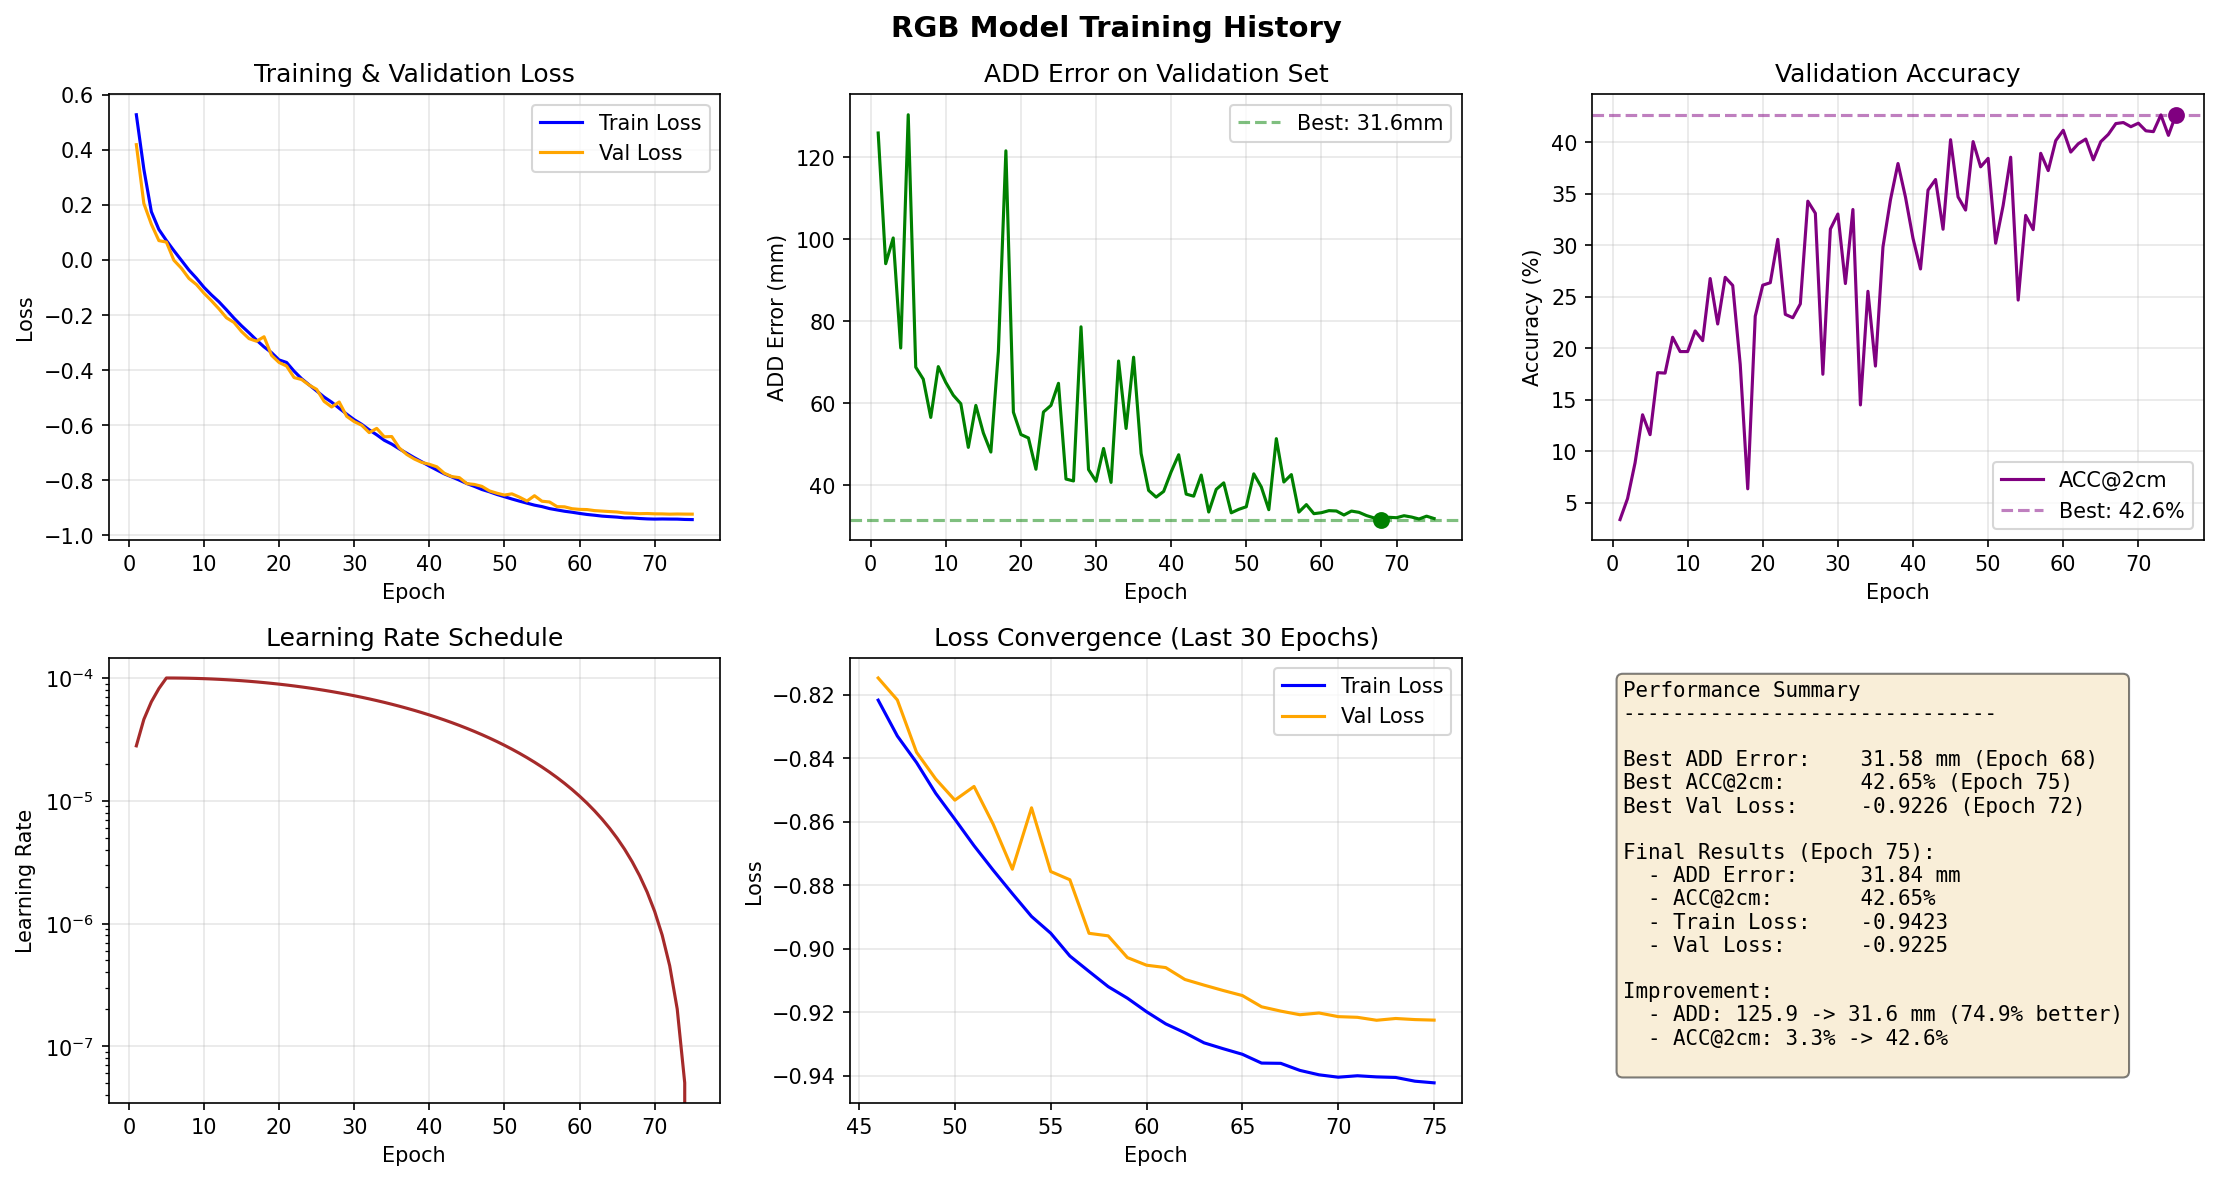
\includegraphics[width=\textwidth]{sec/figures/RGB.png}
    \caption{RGB model training curves showing loss convergence, ADD error, accuracy, and learning rate schedule.}
    \label{fig:training_rgb}
\end{figure*}
\subparagraph{Optimization.}
We use AdamW~\cite{loshchilov2019adamw} optimizer, which decouples weight decay from the gradient update. Unlike standard Adam with L2 regularization, AdamW applies weight decay directly to the weights, providing more effective regularization for transfer learning from pretrained backbones. This is particularly important for our modified ResNet-50 where we want to regularize all weights uniformly while preserving the pretrained feature extractors.

\begin{center}
\begin{tabular}{l|c}
\textbf{Hyperparameter} & \textbf{Value} \\
\hline
Optimizer & AdamW \\
Learning rate & $1 \times 10^{-4}$ \\
Weight decay & $1 \times 10^{-4}$ \\
Batch size & 48 \\
Epochs & 75 \\
Gradient clipping & max\_norm=1.0 \\
\end{tabular}
\end{center}

\subparagraph{Learning Rate Schedule.}
We employ a two-phase schedule:
\begin{enumerate}
    \item \textbf{Warmup (epochs 1-5):} Linear warmup from 10\% to full learning rate.
    \item \textbf{Decay (epochs 6-75):} Cosine annealing to near zero.
\end{enumerate}

\subparagraph{YOLOv8 Training.}
YOLOv8n-seg (nano variant, pretrained on COCO) is fine-tuned on LineMOD for object detection and instance segmentation:

\begin{center}
\begin{tabular}{l|c}
\textbf{Parameter} & \textbf{Value} \\
\hline
Base model & YOLOv8n-seg (COCO) \\
Epochs & 50 \\
Image size & 640$\times$640 (from 640$\times$480) \\
Batch size & 48 \\
Optimizer & AdamW (lr=0.001) \\
Early stopping & patience=20 \\
\end{tabular}
\end{center}

The fine-tuned model achieves \textgreater 95\% mAP50 on LineMOD test set, providing reliable detection and segmentation masks for the pose estimation stage. Training takes approximately 1 hour on a single GPU.

\subparagraph{Training Curves.}

\cref{fig:training_rgb} shows the RGB model training history. The model converges to 42.6\% validation ACC@2cm with 31.6mm ADD error (final test set: 41.2\%, 31.5mm).

\cref{fig:training_rgbd} shows the RGBD model training history. The model achieves 84.5\% validation ACC@2cm with 13.9mm ADD error (final test set: 84.9\% ACC, 13.5mm ADD)---a significant improvement over the RGB model due to the depth prior.

\begin{figure*}[t]
    \centering
    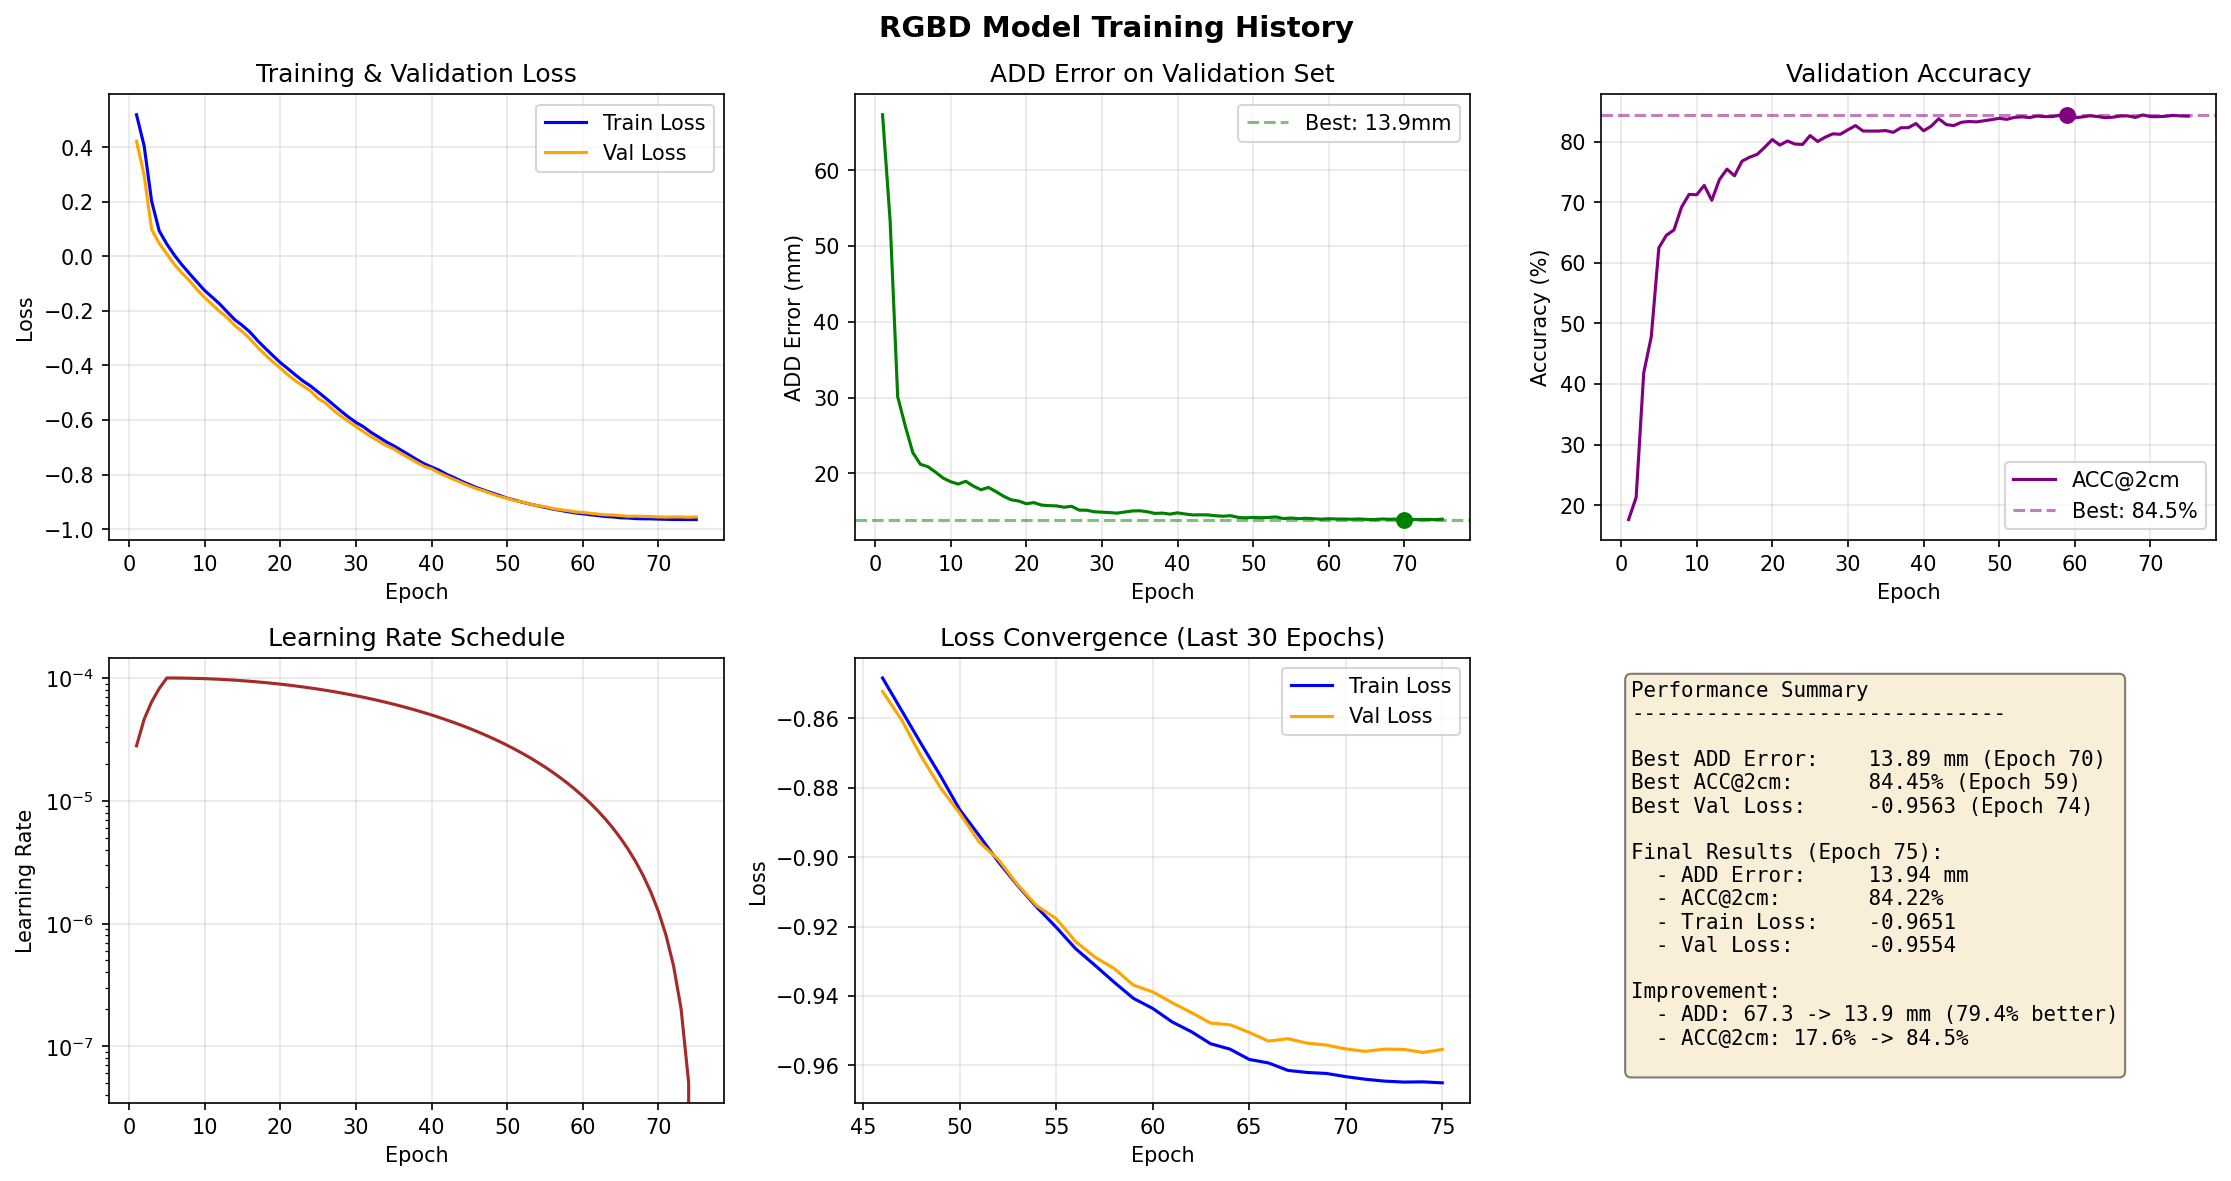
\includegraphics[width=\textwidth]{sec/figures/RGBD.png}
    \caption{RGB-D model training curves. The depth information enables faster convergence and significantly better final accuracy.}
    \label{fig:training_rgbd}
\end{figure*}

\subsection{Testing}

\paragraph{Evaluation Loss (ADD Metric).}

Unlike training losses which measure rotation and translation separately, evaluation uses the ADD (Average Distance of Model Points) metric which measures the actual 3D pose error:
\begin{equation}
    \text{ADD} = \frac{1}{m}\sum_{i=1}^{m} \|(\mathbf{R}_{pred} \mathbf{p}_i + \mathbf{t}_{pred}) - (\mathbf{R}_{gt} \mathbf{p}_i + \mathbf{t}_{gt})\|_2
\end{equation}
where $\{\mathbf{p}_i\}_{i=1}^m$ are $m=500$ downsampled 3D model points. Note: ADD is also computed during training on the validation set for monitoring purposes, separate from the training loss used for backpropagation.

\subparagraph{ADD-S (for Symmetric Objects).}
For objects with rotational symmetry (eggbox, glue), we use closest point matching:
\begin{equation}
    \text{ADD-S} = \frac{1}{m}\sum_{i=1}^{m} \min_{j} \|(\mathbf{R}_{pred} \mathbf{p}_i + \mathbf{t}_{pred}) - (\mathbf{R}_{gt} \mathbf{p}_j + \mathbf{t}_{gt})\|_2
\end{equation}

\subparagraph{ADD-2cm Accuracy.}
A pose is considered correct if ADD (or ADD-S) is less than 20mm.

\paragraph{Inference Pipeline.}
During testing:
\begin{enumerate}
    \item YOLOv8 detects and segments objects in the input image
    \item For each detection, extract crop and run pose model
    \item Compute ADD/ADD-S against ground truth
\end{enumerate}
